\NeedsTeXFormat{LaTeX2e}
\documentclass[11pt, DIV=26,a4paper]{scrartcl}
\usepackage[utf8]{inputenc}
\usepackage{librefranklin}
\usepackage{libertine}
\usepackage[T1]{fontenc}
\usepackage{pifont}
\usepackage{xifthen}
\usepackage{etoolbox}
\usepackage{eso-pic}
\usepackage{xspace}
\usepackage{enumitem}
\usepackage{graphicx}
\usepackage{tabularx}
\usepackage{multirow}
\usepackage[absolute]{textpos}
\usepackage{tikz}
\usepackage[french, british]{babel}
\usepackage{datetime2}
\usepackage{xcolor}
\usepackage[%
		backend=biber,%
		style=ext-alphabetic-verb,%
		articlein=false,%
		firstinits=true,%
		date=year,%
		useprefix=false,%
		]{biblatex}
\addbibresource{mypub.bib}
\usepackage[hidelinks]{hyperref}
\usepackage{ocgx2}

\newif\iflangfrench
\langfrenchfalse
\newcommand{\checklang}[2]{%
	\ifthenelse{\boolean{langfrench}}{#2}{#1}%
}
\iflangfrench
\selectlanguage{french}
\fi
\DeclareRobustCommand{\india}{\checklang{India}{Inde}\xspace}
\newcolumntype{M}{>{\hsize=.5\hsize\linewidth=\hsize\bfseries\raggedleft\arraybackslash}X}
\newcolumntype{D}{>{\hsize=1\hsize\linewidth=\hsize\raggedright\arraybackslash}X}

\setlength{\TPHorizModule}{1 cm}
\setlength{\TPVertModule}{1 cm}

\AtBeginEnvironment{description}{\small}
\begin{document}
\begin{tikzpicture}[overlay, remember picture]
	\node[yshift=5mm, xshift=-2.5cm] at (current page.south east) {\textcolor{gray}{\scriptsize \checklang{last modified on  }{dernière modification au} \today}};
\end{tikzpicture}
\setlength{\parindent}{0pt}
\setkomafont{section}{\Large\bfseries\sffamily\MakeUppercase}
\setlist{nosep}
\pagestyle{empty}
\begin{center}
{	\huge \textsf{Giridhar \textbf{Kulkarni}}
} \\[1ex]
\href{https://codegiri.github.io/webpage}{\textcolor{gray}{https://codegiri.github.io/webpage}}
\\
\textcolor{gray}{\scriptsize%
\begin{tabular}{c|c|c}
	Inspire: \href{https://inspirehep.net/authors/1727127}{G.Kulkarni.3}
	&
	ResearchGate: \href{https://www.researchgate.net/profile/Giridhar_Kulkarni3}{Giridhar\_Kulkarni3}
	&
	LinkedIn: \href{https://www.linkedin.com/in/giridhar-k-55456570}{giridhar-k-55456570}
	%& | &
	%ORCID: \href{https://orcid.org/0000-0001-8354-3120}{0000-0001-8354-3120}
\end{tabular}
}
\end{center}
\rule[1em]{\linewidth}{.4pt}%
\vspace{-1em}
\rule[1em]{\linewidth}{1pt}
%
\begin{minipage}{0.74\textwidth}
\begin{tabularx}{1\textwidth}{M | D}
	\checklang{Date of birth}{Date de naissance}	&	27\checklang{\textsuperscript{th} September}{ septembre} 1993
	\\
	\checklang{Place of birth}{Lieu de naissance}	&	Ahmednagar, \textsc{\india}
\end{tabularx}
\begin{tabularx}{1\textwidth}{M | D}
	\checklang{Nationality}{Naltionalité}		&	\checklang{Indian}{Indienne}
	\\
	\checklang{Civil status}{État civil}		& 	\checklang{Unmarried, without children}{célibataire, sans enfants}
\end{tabularx}
\\[.5em]
\begin{tabularx}{1\textwidth}{M | D}
	\checklang{Current residence}{Domicile actuel}	& 	Dijon 21000, \textsc{France}
\end{tabularx}
\begin{tabularx}{1\textwidth}{M | D}
	\checklang{Mobile phone no.}{n\textsuperscript{o} de tél. portable}	&	\href{tel:+33783296075}{+33\space\textperiodcentered\space 7 83 29 60 75}
\end{tabularx}
\begin{tabularx}{1\textwidth}{M | D}
	\multirow[c]{1}{*}{\checklang{Email addresses}{courriels}}					%&	\href{mailto:giridhar.kulkarni@u-bourgogne.fr}{giridhar.kulkarni@u-bourgogne.fr}

	%\\
			&	\href{mailto:giridhar.kulkarni@protonmail.ch}{giridhar.kulkarni@protonmail.ch}
\end{tabularx}
\end{minipage}
\begin{minipage}{.24\textwidth}
	\raggedleft
	\fbox{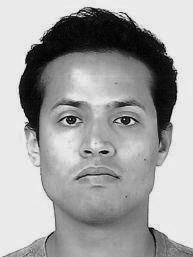
\includegraphics[height=4.5cm]{photo.png}}
\end{minipage}
%
\\[1em]
\begin{minipage}{0.74\textwidth}
\checklang{%
\section*{Employment}
}{%
\section*{Expérience professionelle}
}
\begin{tabularx}{\textwidth}{M | D}
	\checklang{University of Burgundy}{Université de Bourgogne}
	21078 Dijon, \textsc{France}
	&
	\checklang{Research and Teachning Assistant (RA/TA)}{Attaché Temporaire d'Enseignement et de Recherche (ATER)}
	\begin{description}[left=0pt]
	\item	\checklang{September 2019 -- August 2020, full-time}{septembre 2019--août 2020, temps-plein}
	\end{description}
	\\[-1em]
	&
	\checklang{Teaching contract}{Vacataire d'enseignement} {\small %
	(\checklang{Janurary 2019 -- Juin 2019}{janvier 2019 -- juin 2019})}
\end{tabularx}
\checklang{%
\section*{Education and Research}
}{%
\section*{Études et Recherches}
}
\begin{tabularx}{\textwidth}{M | D}
	\checklang{University of Burgundy}{Université de Bourgogne}
	21078 Dijon, \textsc{France}
	&
	\checklang{PhD in mathematics}{Doctorat de mathématiques}
	\begin{description}
		\item \checklang{Since October 2016}{en préparation depuis octobre 2016}
		\item \checklang{Thesis defence scheduled on 20\textsuperscript{th} November 2020}{La soutenence est fixé au 20 novembre 2020}
		\item[\checklang{Title:}{Titre :}] \checklang{\mbox{Asymptotic analysis} of the form-factors of the \mbox{quantum spin chains}}{\mbox{Études asymptotiques} des \mbox{facteurs de forme} des \mbox{chaînes de spins}}
		\item[\checklang{Thesis advisor:}{Directeur de thèse :}] \checklang{Nikolai Kitanine}{Nikolaï \textsc{Kitanine}}
	\end{description}%
	\vspace{-1em}
	\\
	\checklang{University of Cergy-Pontoise}{Université de Cergy-Pontoise}, 95011 \textsc{France}
	&
	\checklang{Master in theoretical physics}{Master (M2) de physique théorique}
	\begin{description}
		\item (2015--2016)
		\item[\checklang{Specialisation:}{Spécialité :}] systèmes inégrables 
		\item[\checklang{Project:}{Mémoir :}] \checklang{Algebraic Bethe ansatz}{Ansatz de Bethe algébrique}
		\item[\checklang{Supervisor:}{Maître de stage :}] \checklang{Nikolai Kitanine}{Nikolaï \textsc{Kitanine}}
	\end{description}
	\\
	Indian Institute of Technology, Guwahati 781039, \textsc{\india}
	&
	\checklang{Bachelor of Technology}{Licence en ingénierie}
	\begin{description}
		\item (2011--2015)
		\item[\checklang{Specialisations:}{Specialisations :}] \checklang{Physics, Mathematics}{physique, mathématiques}
		\item[\checklang{Project:}{Mémoir :}] Axionic models for cosmological inflation
		\item[\checklang{Supervisor:}{Maître de stage :}] Arunansu Sil
	\end{description}
	\\
	\checklang{High-school}{École secondaire} & Jawahar Navodaya Vidyalaya, \india (2005--2009)
\end{tabularx}
\end{minipage}
\begin{minipage}{0.25\textwidth}
\vspace*{.5em}
\checklang{%
\section*{Computer Skills}
}{%
\section*{Compétences en informatiques}
}
{\small
\checklang{%
\minisec{Programming}  C, C++, Python
}{%
\minisec{Programmation}  C, C++, Python
}

\checklang{%
\minisec{Computational tools} Mathematica, MATLAB
}{%
\minisec{Outils de calcul} Mathematica, MATLAB
}

\checklang{\minisec{Web development}
}
{
\minisec{Programmation du web}
}
HTML5, CSS, Javascript.

\checklang{%
\minisec{Typesetting}  \LaTeXe, Xe\TeX, pgf/tikz.
}{%
\minisec{Composition} \LaTeXe, Xe\TeX, pgf/tikz
}
\checklang{%
\minisec{OS \& Utilities} arch/debian, Bash, Git, regex
}{%
\minisec{OS \& outils} arch/debian, Bash, Git, regex
}
\checklang{%
\minisec{Photography} GIMP / Adobe Photoshop
}{%
\minisec{Photographie} GIMP / Adobe Photoshop
}
}
%
\checklang{%
\section*{Languages}
}{%
\section*{Langues}
}
\begin{description}
\checklang{%
\item[English] proficient 
}{%
\item[Anglais] courant 
}
\checklang{%
\item[French] advanced 
}{%
\item[Français] niveau avancé
}
\checklang{%
\item[Hindi] second language
}{%
\item[Hindi] seconde langue
}
\checklang{%
\item[Marathi] native speaker
}{%
\item[Marathé] langue maternelle
}
\end{description}
%
\checklang{%
\section*{Hobbies}
}{%
\section*{Loisirs}
}
\vspace{-1em}
\checklang{%
\small
Astronomy, Board games, Cooking, Cycling, Tennis
}{%
\small
astronomie, cuisine, jeux de société, vélo, tennis
}
\end{minipage}
\\
%
\section*{Publications}
\fullcite{KitK19}
\vspace{-1em}
\checklang{%
\paragraph*{Key area of interest: } Quantum integrable systems, Form-factor approach 
}{%
\paragraph*{Centres d'interêt de recherche :}
Systèmes intérgables quantiques, l'approche des facteurs de formes
}
\checklang{%
	\section*{\large Other Campus Activities}
}{%
\section*{\large Autres acitivités sur le campus}
}
\begin{minipage}{0.49\textwidth}
	\begin{itemize}
		\footnotesize
	\item 
		\checklang{%
			Organiser of docotral student seminar (2017--2019) 
		}{%
		responsable des séminaires doctorants (2017--2019)
	}
\item 
	\checklang{%
		Treasury of doctoral student association (2017--2020)
	}{%
	trésorier de l'association des doctorants D.M.D. (2017--2020)
}
\end{itemize}
\end{minipage}
\begin{minipage}{0.49\textwidth}
	\begin{itemize}
		\footnotesize
	%\item
		%\checklang{%
			%Participation to the Messier marathon (2013)
		%}{%
		%participation au marathon Méssier (2013)
	%}
\item 
	\checklang{%
		Coordinator of amateur astronomy club of IIT Guwahati (2012--2013)
	}{%
	animateur dans la société d'astronomie amateur (2012--2013)
}
\end{itemize}
\end{minipage}
\clearpage
\checklang{%
\section*{Teaching}
}{%
\section*{Enseignement}
}
\def\arraystretch{.25}
\begin{tabularx}{\textwidth}{>{\hsize=.2\hsize\linewidth=\hsize\raggedleft\arraybackslash}X | X}
\checklang{%
Spring 2020
}{%
printemps 2020
}
&%
\vspace{-.5em}
\begin{itemize}[itemsep=.5em, left=0em, label=\ding{227}]
\item
\checklang{%
MaIE2A: Maths tutorials for first-year students in electronics \& informatics
}{%
MaIE2A : TD de maths pour les étudiants de L1 en informatiques et électroniques 
}
	\begin{description}
	\item
	\checklang{%
	{\small sequence and series, convergence, system of linear equations, matrices, vector spaces, \textellipsis}
	}{%
	{\small suites et séries, convergence, système linéaires, matrices, espace vectoriel, \textellipsis}
	}
	\end{description}
\item
\checklang{%
MaIE4A: Maths tutorials for second-year students in electronics \& informatics
}{%
MaIE4A : TD de maths pour les étudiants de L2 en informatiques et électroniques 
}
	\begin{description}
	\item
	\checklang{%
	{\small linear algebra: vector spaces, bases, linear maps, rank theorem, diagonalisation; graph theory, electronic circuits, \textellipsis} 
	}{%
	{\small algèbre linéaire : espace vectoriel, bases, application linéaires, théorème du rang, diagonalisation; théorie des réseaux, circuits électroniques, \textellipsis}
	}
	\end{description}
\item
\checklang{
Mathematics for biology
}{%
Mathématiques appliquées à la biologie
}
	\begin{description}
	\item
	\checklang{%
	{\small geometry, derivatives, intergration, modelisation and optimisation}
	}{%
	{\small geometrie, derivées, intergration, modelisation et optimisation}
	}
	\end{description}
\end{itemize}
\\
\checklang{%
Autumn 2019
}{%
automne 2019
}
&%
\vspace{-.5em}
\begin{itemize}[left=0em, label=\ding{226}, itemsep=.5em]
\item
\checklang{%
Tutotirals for `mathematical methods of quantum mechanics' (masters program)
}{%
TD du M1 math.ph. : `Mathematical Methods of Quantum Mechanics'
}
	\begin{description}
	\item
	{\small reduced density matrix, Van Neuman entropy, entanglement, harmonic oscillator, one-dimensional portential well, interacting spin systems, oscillator chain, \textellipsis}
	\end{description}
\item
\checklang{%
Math3A: Tutorials on analysis for second-year students in mathematics 
}{%
Math3A : TD d'analyse pour les étudiants en L2 de maths
}
	\begin{description}
	\item
	\checklang{%
	{\small sequences: monotonocity, convergence, Cauchy sequence, subsequences; series: absolute convergence, Riemann series, Abel transform, alternating series, power series}
	}{%
	{\small suits: monotonicité, convergence, suite de Cauchy, suites éxtraites; séries: convergence absolu, série de Riemann, transform d'Abel, séries alternées, séries entiers}
}
	\end{description}
\item
\checklang{%
MaPC1A: Maths tutorials for first-year students in physics and chemistry 
}{%
MaPC1A : TD de maths pour les étudiants en L1 physique et chimie
}
	\begin{description}
	\item
	\checklang{%
	{\small fonctions, limits, continuity, derivation, integration, Taylor series \textellipsis}
	}{%
	{\small fonctions, limites, continuité, dérivation, intégration, développement limités, \textellipsis}
	}
	\end{description}
\item
\checklang{%
MaIE1A: Maths tutorials for first-year students in informatics and electronics
}{%
MaIE1A : TD de maths pour les étudiants de L1 en informatiques et électroniques
}
	\begin{description}
	\item
	\checklang{%
	{\small complex numbers, fonctions, continuity, derivation, integration}
	}{%
	{\small nombres complexes, fonctions, continuité, dérivation, intérgation}
	}
	\end{description}
\item 
\checklang{%
Mathematics for second-year economy students
}{%
Maths pour l'économie
}
	\begin{description}
	\item
	\checklang{%
	{\small system of linear equations, matrices, rank theorem, optimisation problems, \textellipsis}
	}{%
	{\small système des équation linéaires, matrices, théorème du rang, problèmes d'optimisations, \textellipsis}
	}
	\end{description}
\end{itemize}
\\
\checklang{%
Spring 2019
}{%
printemps 2019
}
&%
\vspace{-.5em}
\begin{itemize}[itemsep=0.5em, left=0em, label=\ding{227}]
\item
\checklang{%
MaIE4A: Maths tutorials for second-year students in electronics \& informatics
}{%
MaIE4A : TD de maths pour les étudiants de L2 en informatiques et électroniques 
}
	\begin{description}
	\item
	\checklang{%
	{\small linear algebra: vector spaces, bases, linear maps, rank theorem, diagonalisation; combinatorics, graph theory \textellipsis} 
	}{%
	{\small algèbre linéaire : espace vectoriel, bases, application linéaires, théorème du rang, diagonalisation; combinatoires; théorie des réseaux}
	}
	\end{description}
\item
\checklang{
Mathematics for biology
}{%
Mathématiques appliquées à la biologie
}
	\begin{description}
	\item
	\checklang{%
	{\small geometry, derivatives, intergration, modelisation and optimisation}
	}{%
	{\small geometrie, derivées, intergration, modelisation et optimisation}
	}
	\end{description}

\end{itemize}
\end{tabularx}
%
%\checklang{%
%\section*{Seminars \& Conferences}
%}{%
%\section*{Séminaires \& conférences}
%}
\checklang{%
\section*{Conferences}
}{%
\section*{Conférences}
}
\begin{itemize}[left=0pt, itemsep=.5em, label=\ding{111}]
\item 
\checklang{%
\textbf{Bourgogne-Franch Comté Research Federation Annual Meeting}%
}{%
\textbf{Journée de la fédération de recherche de Bourgogne-Franche Comté}%
}%
, Besançon, \textsc{France}
\checklang{%
(Oct 2019)
}{%
(oct 2019)
}
\begin{description}
	\checklang{%
	\item[Title of presentation:]
	Exact computations of form-factors for quantum spin chains
	}{%
	\item[Titre de l'exposée : ]
	Calculs exactes des facteurs de formes des chaînes de spins
	}
\end{description}
\item
\checklang{%
\textbf{Young researchers meeting on integrable systems}%
}{%
\textbf{Conférence pour les jeunes chercheurs en systèmes intégrables}
}%
, Cergy-Potoise, \textsc{France}
\checklang{%
(June 2019)
}{%
(juin 2019)
}%
\item
\checklang{%
\textbf{Les Houches summar school on integrability in atomic and condensed matter physics}%
}{%
\textbf{École d'été des Houches sur \textit{Integrability in atomic and condensed matter physics}}%
}
, École de physique des Houches, Les Houches, \textsc{France}
(August 2018)
\item
\checklang{%
\textbf{Correlation functions in quantum integrable systems and beyond}%
}{%
\textbf{Fonctions de corrélation dans système intégrables quantique et au-delà}%
}%
, ENS de Lyon, \textsc{France}
\checklang{%
(Octobre 2017)
}{%
(octobre 2017)
}
\item
\checklang{%
\textbf{GGI Winter school on Statistical Field Theories (SFT)}%
}{%
\textbf{École d'hiver de GGI sur \textit{Statistical Field Theories} (SFT)}%
}%
, Florence, \textsc{Italy}
\checklang{%
(February 2017)
}{%
(février 2017)
}
\item
\checklang{%
\textbf{ICTS Winter School on Knot theory and topology}%
}{%
\textbf{École d'hiver de ICTS sur la théorie des nœuds et topologie}%
}{%
}%
, Mohali, \textsc{\india}
\checklang{%
(Decembre 2014)
}{%
(décembre 2014)
}
\end{itemize}
%
\checklang{%
\section*{Seminars}
}{%
\section*{Séminaires}
}
\begin{itemize}[left=0pt, itemsep=.5em, label=\ding{111}]
\item
\checklang{%
\textbf{Doctoral students seminar}%
}{%
\textbf{Sémiraires des doctorants}%
}%
, IMB Dijon, \textsc{France}
\checklang{%
(January 2020)
}{%
(janvier 2020)
}%
\begin{description}
	\checklang{%
	\item[Title of the talk:] Exact lattice models in two-dimensional statistical physics
	}{%
	\item[Titre de l'éxposée :] Modèles exactes du réseaux de deux-dimension dans la physique stastique
	}
\end{description}
\item
\checklang{%
\textbf{Annual Carnot-Pasteur doctoral school day}%
}{%
\textbf{Journée de l'école doctoral Carnot-Pasteur}%
}%
, Dijon, \textsc{France}
\checklang{%
(June 2019)
}{%
(juin 2019)
}%
\begin{description}
	\checklang{%
	\item[Title of the talk:]
	Algebraic Bethe ansatz and form-factors
	}{%
	\item[Titre de l'exposée :]
	Ansatz de Bethe algébrique et facteurs de formes
	}
\end{description}
\item
\checklang{%
\textbf{Doctoral students seminar}%
}{%
\textbf{Sémiraires des doctorants}%
}%
, IMB Dijon, \textsc{France}
\checklang{%
(March 2019)
}{%
(mars 2019)
}
\begin{description}
	\checklang{%
	\item[Title of the talk:] Algebraic Bethe ansatz
	}{%
	\item[Titre de l'exposée :] Ansatz de Bethe algébrique
	}
\end{description}
\item
\checklang{%
\textbf{Annual Carnot-Pasteur doctoral school day}%
}{%
\textbf{Journée de l'école doctoral Carnot-Pasteur}%
}%
, Dijon, \textsc{France}
\checklang{%
(June 2018)
}{%
(juin 2018)
}%
\begin{description}
	\checklang{%
	\item[Title of the talk:]
	Classical and quantum integrability
	}{%
	\item[Titre de l'exposée :]
	Intégrabilité classique et quantique
	}
\end{description}
\item
\checklang{%
\textbf{Young researchers meeting of the UBFC}%
}{%
\textbf{Journée des jeunes chercheurs de l'UBFC}%
}%
, Besançon, \textsc{France}
\checklang{%
(April 2018)
}{%
(avril 2018)
}%
\begin{description}
	\checklang{%
	\item[Title of the talk:]
	Classical and quantum integrability
	}{%
	\item[Titre de l'exposée :]
	Intégrabilité classique et quantique
	}
\end{description}
\end{itemize}
%
\end{document}
